% !TeX spellcheck = en_US
\documentclass[letterpaper,12pt,twoside]{report}
\usepackage{fancyhdr}
\usepackage{fullpage}
\usepackage{tikz}
\usepackage{amsmath}

\begin{document}
	\pagestyle{fancy}
	\fancyhf{}
	\fancyhead[L]{Day 21}
	\fancyhead[R]{\textit{The Calendar Project}}
	\fancyfoot[L]{Citations Involved: ???}
	
	% Problem
	\paragraph{Problem}
	\begin{quote}
		\textsf{There exist many points inside a
			triangle such that segments can be drawn
			from the point to the sides of the triangle
			(not at the vertices) so that the three
			resulting quadrilaterals have equal areas.
			There is only one point inside a triangle
			such that the segments drawn to the
			vertices create three quadrilaterals of
			equal area. How is the point determined?}
	\end{quote}
	
	% Graphics
	\begin{center}
		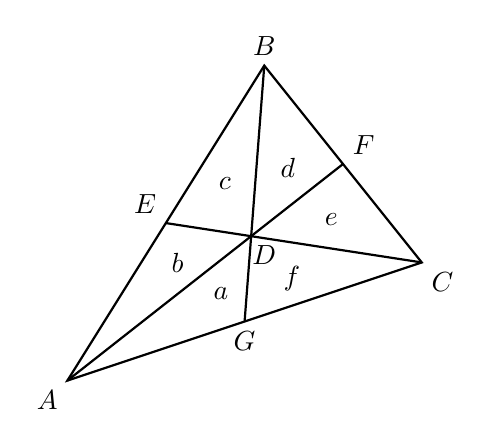
\begin{tikzpicture}[scale=0.5]
		\draw[thick] (-5,-5) -- (0,3) -- (4,-2) -- cycle;
		\draw[thick] (0,3) -- (-0.5,-3.5);
		\draw[thick] (4,-2) -- (-2.5,-1);
		\draw[thick] (-5,-5) -- (2,0.5);
		
		\node[below left] at (-5,-5) {$A$};
		\node[above] at (0,3) {$B$};
		\node[below right] at (4,-2) {$C$};
		\node at (0,-1.8) {$D$};
		\node[above left] at (-2.5,-1) {$E$};
		\node[above right] at (2,0.5) {$F$};
		\node[below] at (-0.5, -3.5) {$G$};
		
		\node at (-1.1,-2.8) {$a$};
		\node at (-2.2,-2) {$b$};
		\node at (-1,0) {$c$};
		\node at (0.6,0.4) {$d$};
		\node at (1.7,-0.9) {$e$};
		\node at (0.7,-2.4) {$f$};
		
		\end{tikzpicture}
	\end{center}
	
	% Reasoning
	\paragraph{Reasoning}
	\begin{quotation}
		
		Consider $\triangle ABC$ above with $D$ being the point described in the problem. Segments $\overline{DB}$, $\overline{DA}$, and $\overline{DC}$ connect $D$ to the vertices of $\triangle ABC$; each is extended from $D$ to the opposite side of the vertex to which they connect. Let $[\triangle ADG]$ be $a$, $[\triangle CDG]$ be $f$, $[\triangle CDF]$ be $e$, $[\triangle BDF]$ be $d$, $[\triangle BDE]$ be $c$, and $[\triangle ADE]$ be $b$.
		
		The three quadrilaterals created by these segments are $ABDC$, $ADBC$, and $ADCB$. These are given to have the same area: $[ABDC]=[ADBC]=[ADCB]$. By the Area Addition Postulate, $[ABDC]+d+e=[ADBC]+b+c=[ADCB]+a+f=[\triangle ABC]$. By substitution, $[ABDC]+d+e=[ABDC]+b+c=[ABDC]+a+f=[\triangle ABC] \Rightarrow d+e=b+c=a+f$. $a+(b+c)=(d+e)+a=d+e+(b+c)-f$; $(b+c)+d=(a+f)+d$; $c+(d+e)=(a+f)+c$.
		
	\end{quotation}
	
	\paragraph{External References}
	
	\begin{enumerate}
		\item ???
	\end{enumerate}
	
\end{document}